\section{数据处理}
\subsection{数据获取}
通过Python爬虫获取了1月20日至今的疫情数据。
\par
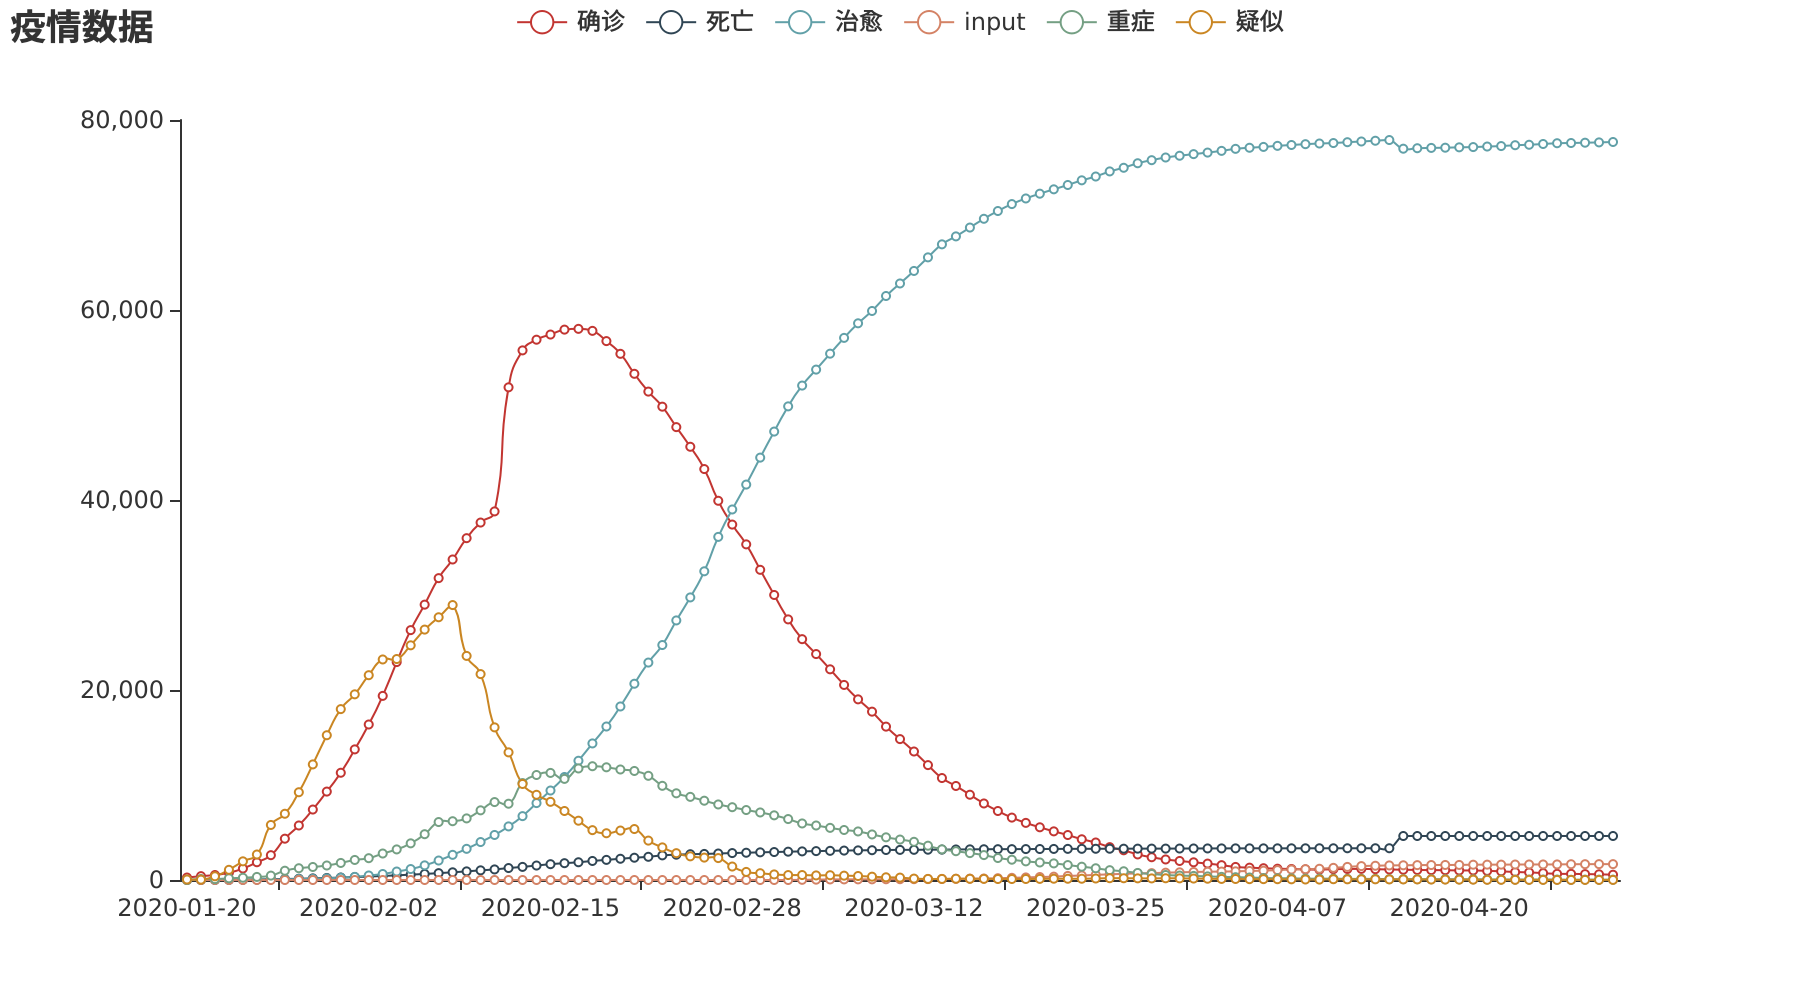
\includegraphics[width=\imagewidth]{疫情数据.png}
\subsection{数据分析}
对数据进行简单的处理,得到每日新增人数曲线。\\
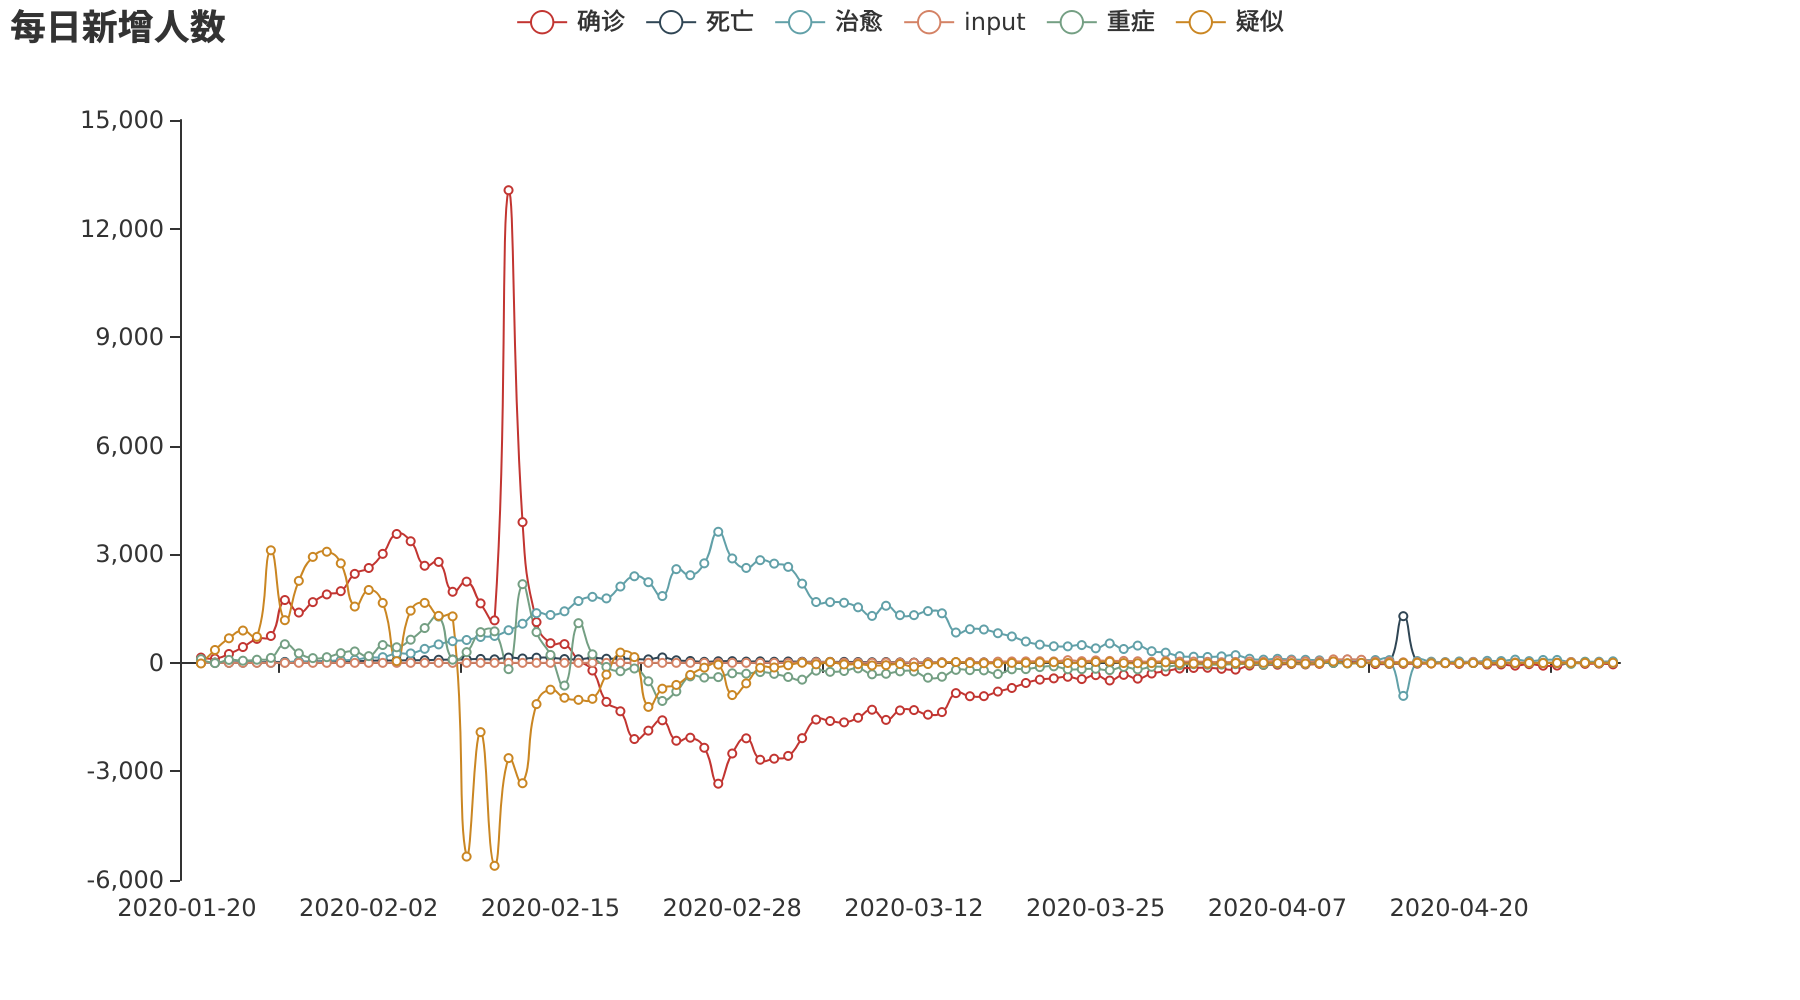
\includegraphics[width=\imagewidth]{每日新增人数.png}
\par
对数据进行简单的观察,可以得到几点:
\begin{itemize}
    \item
          2月12日确诊人数猛增,
          这是因为重新规定了确诊条件,
          导致许多人被纳入确诊人数。
    \item
          治愈曲线比确诊曲线和疑似曲线明显滞后。
\end{itemize}
